% FLOWING (for HPCA'2006)
%
%\documentclass[10pt,dvips]{article}
\documentclass[10pt,dvips]{article}
%\documentclass[10pt,twocolumn,dvips]{article}
\usepackage[english]{babel}
\usepackage{epsfig}
%\usepackage{fancyheadings}
%\usepackage[T1]{fontenc}
%\usepackage[latin1]{inputenc}
%\usepackage{twocolumn}
\usepackage{verbatim,moreverb,doublespace}
%\usepackage{rotate,lscape,dcolumn,array,rotating,latexsym}
%
%\input{epsf}
%
% for (IEEE single-column format)
%\textwidth 6.875in
%\textheight 8.875in
%\topmargin -0.6in
%\oddsidemargin 0mm
%\evensidemargin 0mm
%
% for HPCA (IEEE two-column format)
%\textwidth 6.5in
%\textheight 8.875in
%\topmargin -0.4in
%\oddsidemargin 0mm
%\evensidemargin 0mm
%
% for HPCA;2006
\textwidth 6.5in
\textheight 8.875in
\topmargin -0.4in
\oddsidemargin 0mm
\evensidemargin 0mm
%
%
% turn the following (linespread) on to 1.6 for "double space"
%\linespread{1.6}
%
%
% some publishers want no page numbers for final print
%\pagestyle{empty}
%
\begin{document}
%
%
\title{A microarchitectural proposal for more aggressive 
exploitation of instruction level parallelism}
%
%
\author{
undisclosed
}
%
%
% some publishers do not want a data in the final print
\date{18th July 2005}
%
\maketitle
%
% uncomment the following for first page with no page number (for IEEE)
%\thispagestyle{empty}
%
%
\begin{abstract}
%
We present a new processor microarchitecture for managing aggressive
parallel and speculative instruction execution.  The goal is to explore
ways to maximize processor performance for otherwise general purpose
serial sequential program codes which do not lend themselves to explicit
parallelization efforts.  Instructions are fetched and dispatched for
speculative execution as machine resources are available without first
determining control or data dependencies.  Rather, input dependencies are
determined dynamically at execution time.  Instructions remain in the
processor (without being re-fetched or re-dispatched) and in a state of
readiness for re-execution as correct input dependencies are determined.
Committed instructions provide outputs to speculative instructions, which
in turn re-execute as necessary in order to eventually converge on the
correct committed program state.  We present results showing some
performance gains
over more conventional processor microarchitectures with approximately
equivalent hardware resources when executing integer sequential codes.
Our proposed microarchitecture also features 
interconnection requirements that can be more naturally spatially
separated than those of conventional superscalars.
This lends the microarchitecture to a more
distributed physical implementation, possibly allowing
for larger physically scaled processors in the future.
%
\end{abstract}
%
%
\vspace{-0.15in}
%\vspace{-0.25in}
\section{Introduction}
%\vspace{-0.15in}
%
Although many high performance applications today
can be parallelized at the application level 
and executed on tiled or clustered systems,
there are and will continue
to be requirements for achieving the highest performance
on single threaded highly serially dependent program codes.
We attempt to target this application problem space
through the extraction of instruction level parallelism (ILP).
The prospect of increased numbers of transistors 
available in silicon represents an opportunity to capitalize on
the remaining ILP latent in even sequential (stubbornly non-parallelizable)
programs.
With limits to performance improvement through clock cycle reduction
alone (witness also the recent flattening of higher clock frequencies),
methods such as more aggressive ILP extraction in the microarchitecture
become even more attractive.

Several studies into the limits of instruction level 
parallelism have shown that there is 
a significant amount of parallelism within
typical sequentially oriented single-threaded programs
(e.g., SpecInt-2000).  
The work of researchers including 
Lam and Wilson~\cite{Lam92},
Uht and Sindagi~\cite{Uht95},
Gonzalez and Gonzalez~\cite{Gon97}
have shown that there exists a great amount of instruction level
parallelism that is not being exploited by any existing
computer designs.
Generally, ILP extraction is achieved by introducing multiple
execution units into the microarchitecture and allowing each unit
to operate as independently and as parallel as possible, yielding
increased instructions per clock (IPC).
One of the key problems with the addition of more parallel hardware
resources
is how to interconnect them in an efficient manner.
Maintaining binary compatibility with existing instruction
set architectures (ISA) is also generally a requirement, so we
target this as well with our proposal.

Microarchitectures such as RAW~\cite{waingold97,taylor02}
or conventional cluster-based systems
address the issue of parallelism within applications but only do so
by exposing the spatially separated nature of their
parallel-processor systems to the compiler and the application itself.
This approach towards parallelism is an important one but
can only address those applications that can be parallelized at
a fairly coarse level.

Other microarchitectures that have employed the
use of multiple execution units for ILP extraction are the Multiscalar-like
processors~\cite{Sohi95,sundararaman97multiscalar},
the SuperThreaded processor model~\cite{tsai96superthread},
and
the Parallel Execution Window processor model~\cite{kemp96pew}.
The proposed MultiCluster machine model by 
Farkas et al.~\cite{farkas97multicluster} are also in this category.
Nagarajan also proposed a {\em Grid Architecture} of ALUs
connected by an operand network~\cite{Nag01}.  
However, the Multiscalar and Grid or grid-like microarchitectures
also rely on the
coordinated use of the compiler along with a new ISA.
This differentiates these approaches with our own, which can be
applied to any existing ISA.
Although many proposed architectures and requirements for increased parallel
programming of the application offer large potential performance increases
over existing machines and non-parallelized programming styles,
the requirement to provide high performance for existing (and future)
non-parallelized
codes with existing ISAs is likely a requirement for decades to come
(withness the x86 ISA for example).

A microarchitecture that bears some similarity with our present
proposal is the Ultrascalar design~\cite{henry99}.
That proposal employed a relatively involved operand interconnection
network (although logarithmic in scale to the size of the
instruction window) that was switched according to 
instruction dependencies so as to route the appropriate input
operand dependency to an instruction and that instruction's
output operand to the appropriate
succeeding instructions.
Our approach avoids the interconnection complexity of the 
Ultrascalar proposal and this is partly
achieved through the dynamic determination of operand dependencies
during execution using a common (not switched) operand forwarding
interconnection fabric.

Our goal is a microarchitecture
that features the benefits of speculative execution with 
relaxed control and data dependencies,
such as done in the proposed Superspeculative 
microarchitecture ~\cite{Lip97}, but with the ability
to managing a large number of instructions simultaneously in flight.
This makes the microarchitecture
suitable for programs normally constrained by short dependency chains.
An important distinction between our proposed microarchitecture and
that of most others is that we dispatch instructions to special structures
resembling reservation stations~\cite{Anderson67,Tom67},
but instead of the instruction
vacating the station upon instruction issue, it
remains in the station until retirement.
Instructions also
dynamically determine their proper input dependencies,
executing and re-executing as needed as new dependencies
are determined.
In our microarchitecture, the traditional reorder buffer (ROB)
is eliminated along with the silicon layout routing complexity
that is associated with it.  
Thus the layout density of implementing
complex associative searches of the ROB for output result updates
is avoided.
These features are all achieved while also using moderately
simple interconnections between our core machine components.
In effect, the centralized functions of both operand dependency determination
in the instruction window
as well as the searching of the ROB for the most recent input operand
is eliminated and instead distributed in our proposal.
This allows for increased physical scalability that is not nearly
as possible with the more conventional
centralized instruction window and ROB-like approaches.

The rest of this paper is organized as follows.
Section 2 gives an overview of the microarchitecture.
Section 3 provides some further details on the more
novel and core components of the microarchitecture.
Section 4 provides some characterization and performance 
results for our microarchitecture through the simulated
execution of benchmark programs.
We summarize in Section 5.
%
\vspace{-0.15in}
%\vspace{-0.25in}
\section{Microarchitecture overview}
%\vspace{-0.15in}
%
%\vspace{-0.25in}
\subsection{Structural overview}
%\vspace{-0.15in}
%
The handling of main memory, and the cache hierarchy 
through the L1 instruction and L1 data caches are all
conventional and similar to existing microarchitectures.
Instruction fetch is also rather conventional.
We also employ: a
load-store-queue (LSQ) component, an architected register file
(containing only committed registers),
structures that closely resemble reservation stations or issue
window slots,
and rather conventional execution function units (FU).
Our adaptation and enhancement of an issue window slot or reservation 
station is termed
an \textit{issue station} (IS).
Figure \ref{fig:overview} shows a high-level block diagram
of our microarchitecture showing the major instruction execution components.
The memory hierarchy, as well as details of the instruction fetch
unit, are not shown as they are similar to those of existing
machines.
%
\begin{figure}
\centering
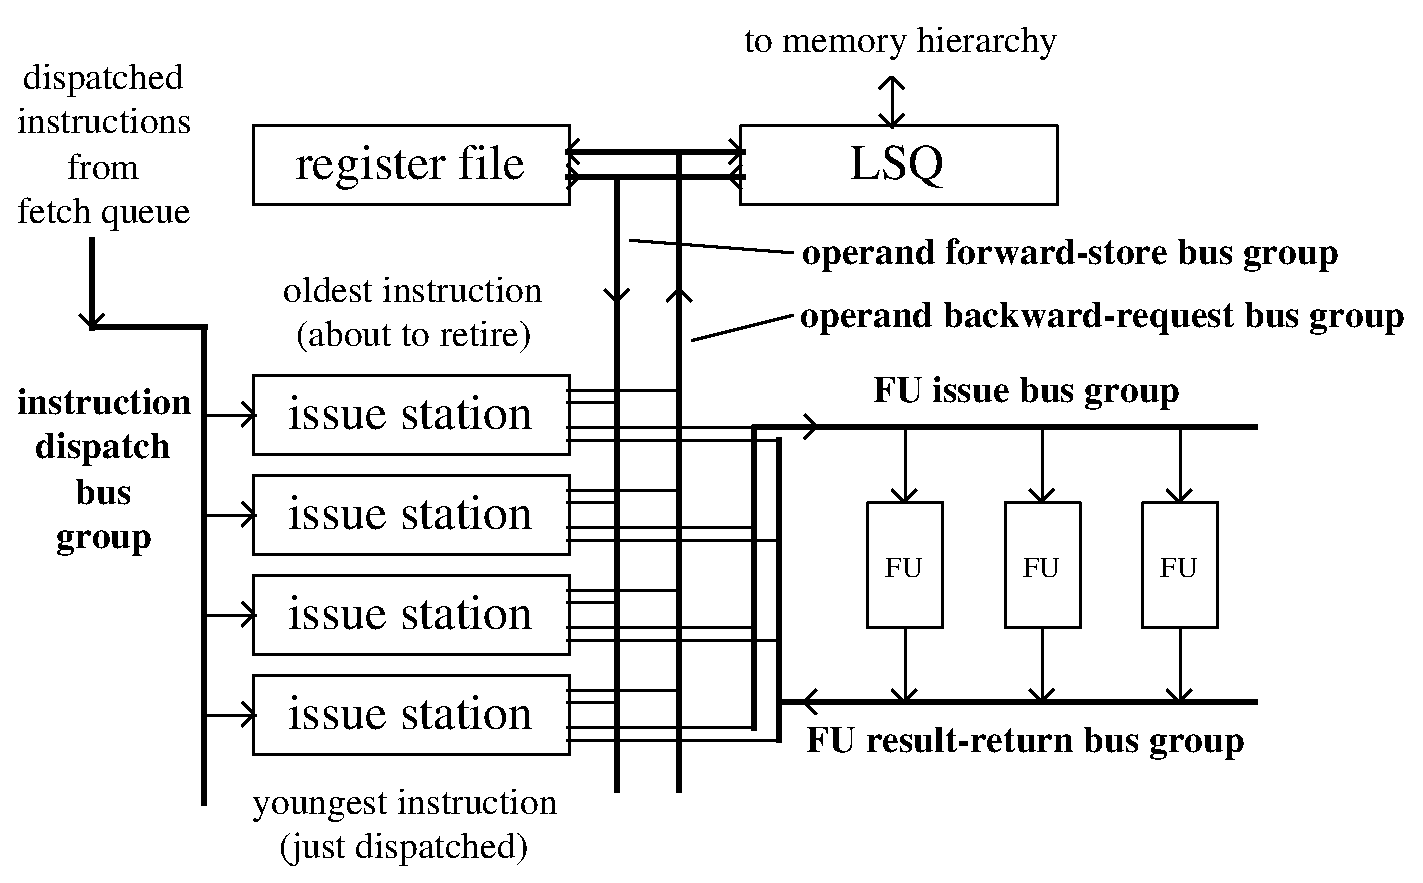
\epsfig{file=figure1.eps,width=3.0in}
\caption{{\em High-level block diagram of our microarchitecture.} 
\small{
Issues stations (IS) are shown on the left and various function
units (FU) on the right.  An architected register file and a
load-store-queue are shown at the top.
Bidirectional operand request and forwarding buses are shown
vertically oriented (to the right of the Issue Stations).
Buses to transport an instruction operation and its source operands
to the function units are also shown. 
Likewise buses to return result operands are present.
}
}
\label{fig:overview}
\end{figure}
%
Although there is only a single load-store-queue (LSQ) and
an architected register file,
the numbers of all other components can
vary with a specific machine implementation.
All ISs are identical, allowing for any
instruction to be dispatched to each.
Function units can be duplicated and functionally differentiated (meaning
different types of units would handle different classes of instructions)
as desired.

Like other machines with reservation stations, we dispatch 
decoded instructions from the fetch unit to these ISs
when one or more of them are empty (available for dispatch) or 
becoming empty on the next clock cycle.  
Instructions are dispatched in-order.
The number of instructions dispatched in any 
given clock cycle is
the lesser of the number of ISs available and the
dispatch width (as counted in numbers of instructions).
Instructions are always dispatched to ISs when
one or more are free (or becoming free) and are generally dispatched
without first knowing their input dependencies or having those
corresponding operands available.

The vertical buses, roughly in the center of Figure \ref{fig:overview},
labeled \textit{operand forward-store} and
\textit{operand backward-request}, are
bidirectional and multi-master bus groups that
allow for operands to be requested from and forwarded to
ISs.
A bus group is a set of one or more buses in parallel 
(the exact number of which is an
implementation option) that
can be used to increase transfer bandwidth through alternative paths.
Bus paths that do not start and end at the same repeater junctions
are also possible and have been explored.
These operand buses (forward-store and backward-request) provide
the means by which instructions acquire their necessary
operands for proper execution.
Requests for operands are generated by ISs and
are placed on the backward-request bus group,
while answers to operand requests are placed on the forward-store bus
group.
Operand requests also travel back
to the register file and LSQ (each also attached to these buses), 
and those units
can likewise forward operands in response to requests.
Operand switching interconnects other than
a bus arrangement are also possible.  
Operands only have
to traverse the operand interconnect arrangement (whatever it might be) in
a single direction ; namely, toward younger dispatched instructions for
forwarded operands and 
toward older dispatched instructions for 
backwarded~\footnote{Perhaps awkward, but consistent with its
opposite of being forwarded.}.
This allows additional flexibility in both the choice of an interconnection
fabric and the ability to electrically isolate segments of
it due to silicon layout propagation delay constraints.

However, 
the simplicity of parallel buses as the basic operand interconnect
generally makes for simpler silicon hardware layout
and better future physical scalability when used in conjunction
with some sort of repeater mechanism.
Our microarchitecture allows for long buses
(longer than the given silicon constraints and propagation
delays) to be split using repeater like units since it
does not assume any fixed delays (in clocks)
for the transfer of operands.  This also effects a great deal of 
flexibility for
both bus and non-bus interconnection arrangements.
The details of how operand bus repeaters work is not discussed
further in this present paper.

Buses are also provided 
for bringing instruction codes and operands from the issue
stations to the FUs and back again.
These are also arranged in a parallel group, the basic group width being
determined by the desired issue width to the FUs.
This arrangement is not too dissimilar to that between the issue window
and the FUs of some conventional microarchitectures.

Collectively, all of the components discussed in this section
(and shown in 
Figure \ref{fig:overview}) are termed the \textit{execution window}.
%
%
%\vspace{-0.25in}
\subsection{Operational overview}
%\vspace{-0.15in}
%
Instructions are decoded after fetch and stored in a buffer (in decoded
form) for possible dispatch to the ISs.
As instructions are dispatch to the ISs, a \textit{time-tag}
is assigned along with the decoded instruction.  
The time-tag is a small positive integer, large enough to represent
the number of ISs in a particular implementation.
New time-tags are assigned sequentially higher values starting from
zero and all time-tags in the execution window are decremented
as instructions commit (effectively decremented by one for each
committed instruction).  This is how time-tag value wrap-around is handled.
This arrangement always keeps higher valued time-tags representing
younger dispatched instructions.  This property is used during the
operand snoop process (described in detail later).
Note that the whole set of ISs effectively
serve the function of the ROB in more conventional machines, albeit
in a more distributed way.

Once instructions are dispatched to ISs,
they issue requests on the backward-request bus group for their input operands.
The ISs then
wait for plausible (generally speculative) input operands
through the process of snooping the operand forward-store bus group.
The process of snooping for operands consists of checking the 
output operands created by other ISs (or forwarded from the
architected register file) to see if they are feasible candidates
to satisfy input dependencies.
Feasible input operands are any of those that have the same architected address.
For register operands, this is the architected number of the register.  
For memory operands it is the architected memory address.
These feasible operands may be from either the
closest older instruction that created a feasible output operand 
or it may be
from still older instructions.  
In the former case the operand
may be speculative or not (depending on whether the instruction
ready to commit or not),
but in the latter case the operand
will generally be speculative but could be the same value as
the proper non-speculative operand by coincidence.
The details of the operand snooping process is
covered in greater detail in a subsequent section.
Issue stations also snoop the backward-request bus group to
see if they have an output operand that may satisfy an outstanding
operand request from a younger IS (determined by time-tag
value).
Note that both the LSQ and the architected register file also
snoop for operand requests (although each only for its particular
operand type).
In this way all operand dependencies are determined dynamically 
during and intermixed with execution or re-execution.
Note that although operands received from the LSQ or architected
register file are always valid (having been committed), 
operands received from older
ISs are generally still speculative.

Once feasible input dependencies have been acquired, the
IS can execute its currently associated instruction.
Some instructions are executed within the IS station itself
while the remaining ones need to 
contend with other ISs for FU availability.
In our present work, the instructions that execute within the
ISs are those with an instruction type of: load-store or
control-flow-change.
With this decision, the logic and state complexity of both the ISs
and the FUs is substantially reduced over
the case where all instructions must proceed through FUs.
Note that typically there is a full add function required by
many or most load-store instructions in order to perform an
address calculation (and the equivalent for comparisons in branch
instructions).
Although this \textit{add} function could be carried out in a
FU, we have chosen to place the adder inside the 
IS.
Although this represents a sizeable silicon resource enhancement
(substantially more transistors) to the IS, it seems
a reasonable decision based on the increasing availability of
transistors with newer technology.
However, this design tradeoff would likely not hold for any CISC-like
ISAs where these instructions are more complex than their
typical RISC definitions.
In general, 
the present arrangement represents a division of execution resources
between both the ISs and the FUs,
effectively increasing issue width.
The process of winning a FU execution-slot constitutes
an instruction issue, in the more conventional sense.
All instruction issues and executions in the machine are entirely out of order.

In the case of requiring an FU for execution, the output results are
transferred back to the IS before being forwarded further.
In both execution type cases,
results of instruction executions are retained within
the IS until retirement.  
Forwarding of instruction execution
results to younger dispatched instructions is 
always done from the IS itself, rather
than from the output of the FUs
(as is often the case in most machines).
This is done since the ISs are the place
where the results are stored as tentative values.
This is consistent with the idea that the ISs are
serving the function of the ROB, which would otherwise
store tentative results.
This also eliminates the requirement for the ISs to
snoop the outputs of the 
FUs for possible new input dependency candidates (dramatically
reducing interconnection requirements).

What has been implicit in the discussion so far is that whenever
operands are snooped by the ISs and are found to be feasible
input dependencies, a re-execution of the associated instruction
may be triggered.
Re-executions do not have to occur if the values of the
input dependencies do not change.
This re-execution technique is somewhat analogous to 
the reply mechanisms being currently proposed,
where an instruction is retained in the issue window and re-issued
if necessary.
However, our proposal presents this idea as
more fundamental to the whole microarchitecture
and more natural as the required input operands 
are immediately present with (located adjacent to)
the instruction to be re-executed (replayed).

Instruction commitment can occur on each clock, is in-order, and
proceeds from the oldest program-ordered
instruction through younger instructions until an instruction
is reached that doesn't meet the requirements for commitment.
Preference to win a FU execution-slot by an issue
station is given to the ISs holding the oldest
dispatched instructions (this facilitates movement towards
commitment).
Instructions can only commit if they have executed at least once,
have not received a new feasible input operand (which could
trigger re-execution and a different committed result),
and are finished forwarding output operands 
to younger dispatched instructions.  
An output operand is considered forwarded when it is placed
on the forward-store bus group.
The last constraint guarantees that all younger
instructions can process the final output operands of older
instructions before those older instructions commit and are
therefore removed from the execution window.
Committed outputs are also forwarded to the architected register
file or LSQ (as appropriate for operand type, register or memory).
Note that instruction commitment is not required to be delayed 
so as to wait for verification that
younger instructions have received their new 
inputs from the committing instruction.
The only requirement for the committing instruction is
that any of their output operands not already forwarded win
a transfer slot on the forward-store bus group.
This
guarantees that the operand will be seen by possibly
dependent instructions.

When a branch is resolved (ready for commitment),
instructions in ISs beyond the resolved branch
are abandoned if they are not on the resolved branch path.
This is similar to what would occur in a microarchitecture
with both an issue window and an ROB, except that both actions
occur in our ISs as opposed to the corresponding
action occurring in both the issue window and the ROB.
Program interrupts and exceptions are handled similarly as they
would in a machine with an ROB.
%
\vspace{-0.15in}
%\vspace{-0.25in}
\section{Core component detail}
%\vspace{-0.15in}
%
%\vspace{-0.25in}
\subsection{Issue Stations}
%\vspace{-0.15in}
%
The ISs provide the most significant distinction of this
microarchitecture from most others.  
These are similar to reservation stations
but contain additional state and logic that allows
for dynamic operand dependency determination as well as
for holding a dispatched instruction (its decoded form) 
until it is ready to be retired.  
There is state inside the station that is relevant to
the instruction itself and specific
to the operands of that instruction (both source and
destination operands).

The state that is primarily associated with the instruction itself
consists of:
%
\begin{itemize}
\vspace{-0.10in}
\item{instruction address}
\vspace{-0.10in}
\item{instruction operation}
\vspace{-0.10in}
\item{execution state}
\vspace{-0.10in}
\item{time-tag}
\vspace{-0.10in}
\item{instruction predication information}
\vspace{-0.10in}
\end{itemize}   
%
The \textit{instruction operation} is derived from the decoded
instruction and specifies the instruction class and other
details needed for the execution of the instruction.
This information may consist of subfields and is generally ISA
specific.
The \textit{instruction address} and \textit{predicate} state
are only used when dynamic predication~\cite{undisclosed2}
is done within the microarchitecture.
The time-tag value is used to order this instruction
with respect to all others that are currently within the execution
window of the machine.
The time-tag is also used as part of the operand snooping
logic (discussed more later).
The \textit{execution state} value constitutes the state
used by various state machines within the IS
for controlling its operation and for determining readiness
for commitment.

The remainder of the state consists of one or more input
source operands and one or more output destination operands.
All operands regardless of type and whether source or destination
occupy a similar structure within an IS, termed an
\textit{operand block}.
More detail on these operand blocks and operand management
is provided in the next section.

A simplified block diagram of our IS is shown in 
Figure \ref{fig:issuestation}.
%
\begin{figure}
\centering
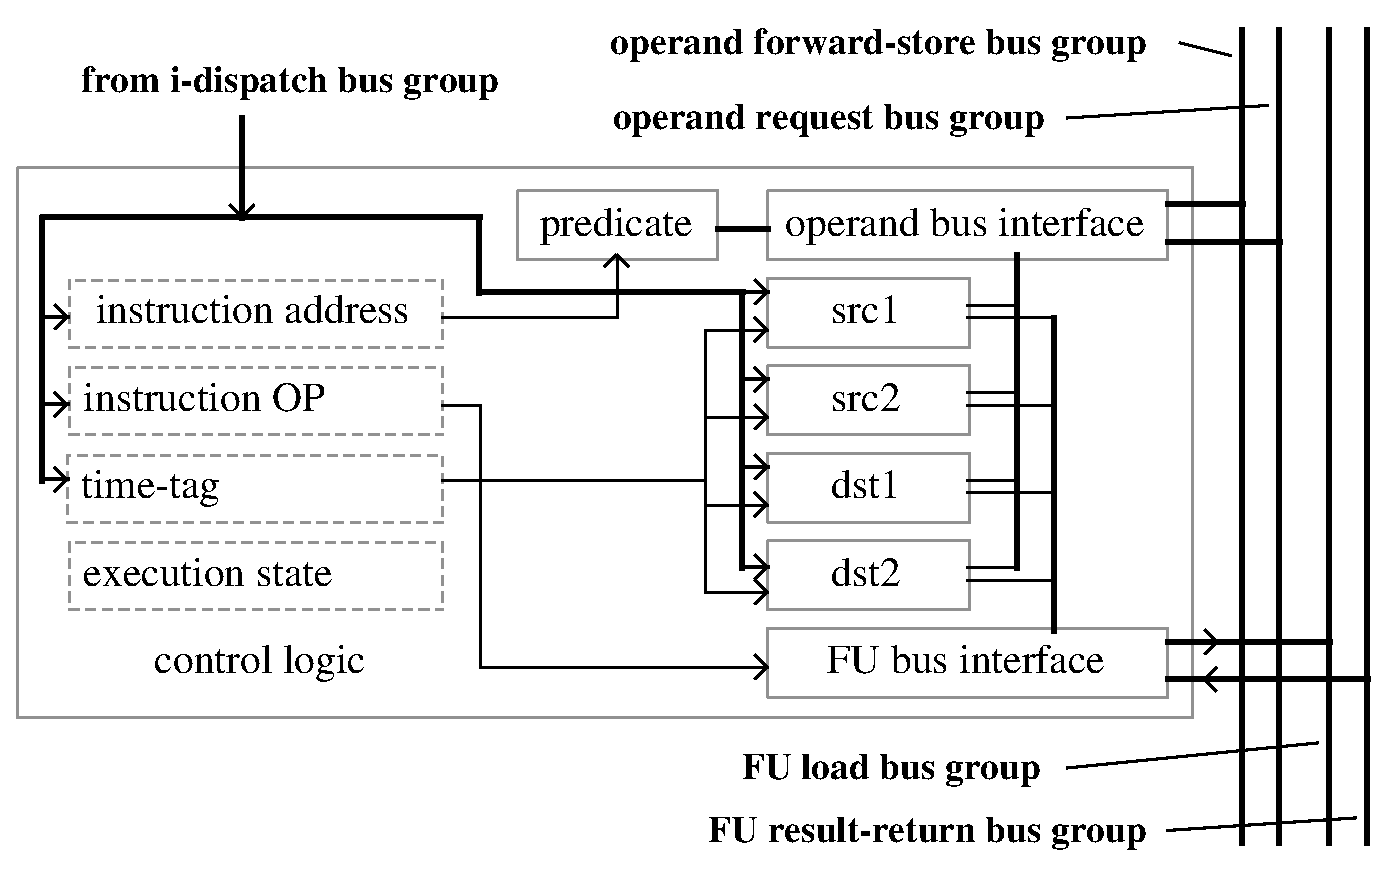
\epsfig{file=figure2.eps,width=3.0in}
\caption{{\em High-level block diagram of our Issue Station.} 
\small{
The major state and sub-blocks associated with an Issue Station is shown.
General instruction state (shown in dash-lined boxes) is
on the left, while
four operand blocks (two source and two destination),
and the four primary bus group interfaces (grouped by function at
upper right and lower right) to the rest of the
execution window are on the right.
}
}
\label{fig:issuestation}
\end{figure}
%
In this example, a total of four operand blocks are shown, labeled:
\textit{src1}, 
\textit{src2}, 
\textit{dst1}, 
and \textit{dst2}.
The number of source and destination operand blocks that are
used for any given machine is dependent upon the requirements
of the ISA implemented.
%
%
%\vspace{-0.25in}
\subsection{Operands}
%\vspace{-0.15in}
%
The types of operands are distinguished: register and memory.
Operands blocks are constructed to hold either type.
The state within an operand block consists of:
%
\begin{itemize}
\vspace{-0.10in}
\item{type of operand}
\vspace{-0.10in}
\item{time-tag}
\vspace{-0.10in}
\item{address}
\vspace{-0.10in}
\item{size}
\vspace{-0.10in}
\item{previous value}
\vspace{-0.10in}
\item{value}
\vspace{-0.10in}
\end{itemize}   
%
The operand \textit{time-tag}
serves
an analogous purpose as the time-tag register within an IS,
except that it applies specifically to this particular
operand rather than to the instruction as a whole.
Again, this time-tag is used in the operand snooping logic
and allowed for the dynamic discovery of dependencies
for instructions.

The \textit{address} field differs
depending on the type of the operand.
For register operands, the address would be
the name of the architected register.
All ISA architected registers are typically provided a
unique numerical address.  These would include the
general purpose registers, any status or other non-general
purpose registers, and any possible ISA (architected) predicate registers
(like those in the iA-64 ISA~\cite{intel99ia,schlansker00epic}.
For memory operands, the identifying address is just the
programmer-visible architected memory address of the corresponding
memory value.

The \textit{size} is only used for memory operands and holds
its size in bytes.
The \textit{value} holds the present value of the operand
calculated from this present instruction (if it has executed
at least once).
The \textit{previous value} is only used for destination
operands and holds the value that the operand
had before it may have been changed by the execution of 
the present instruction.
The previous value is used 
when a forwarded operand with a specific
address was incorrect.
This situation occurs when addresses for memory operands are
speculatively calculated but are later determined to have changed.
An operand with the old address is forwarded with the previous
value to correct the situation.

Figure \ref{fig:operand} shows a simplified block diagram of
an operand block along with its major data paths for its
major functions.  These major functions consist of:
%
\begin{itemize}
\vspace{-0.10in}
\item{snooping for feasible input operands}
\vspace{-0.10in}
\item{snooping for operand requests from elsewhere}
\vspace{-0.10in}
\item{issuing instruction code to FUs (if required due to instruction type)}
\vspace{-0.10in}
\item{receiving FU store-results back (if required due to instruction type)}
\vspace{-0.10in}
\end{itemize}   
%
%
\begin{figure}
\centering
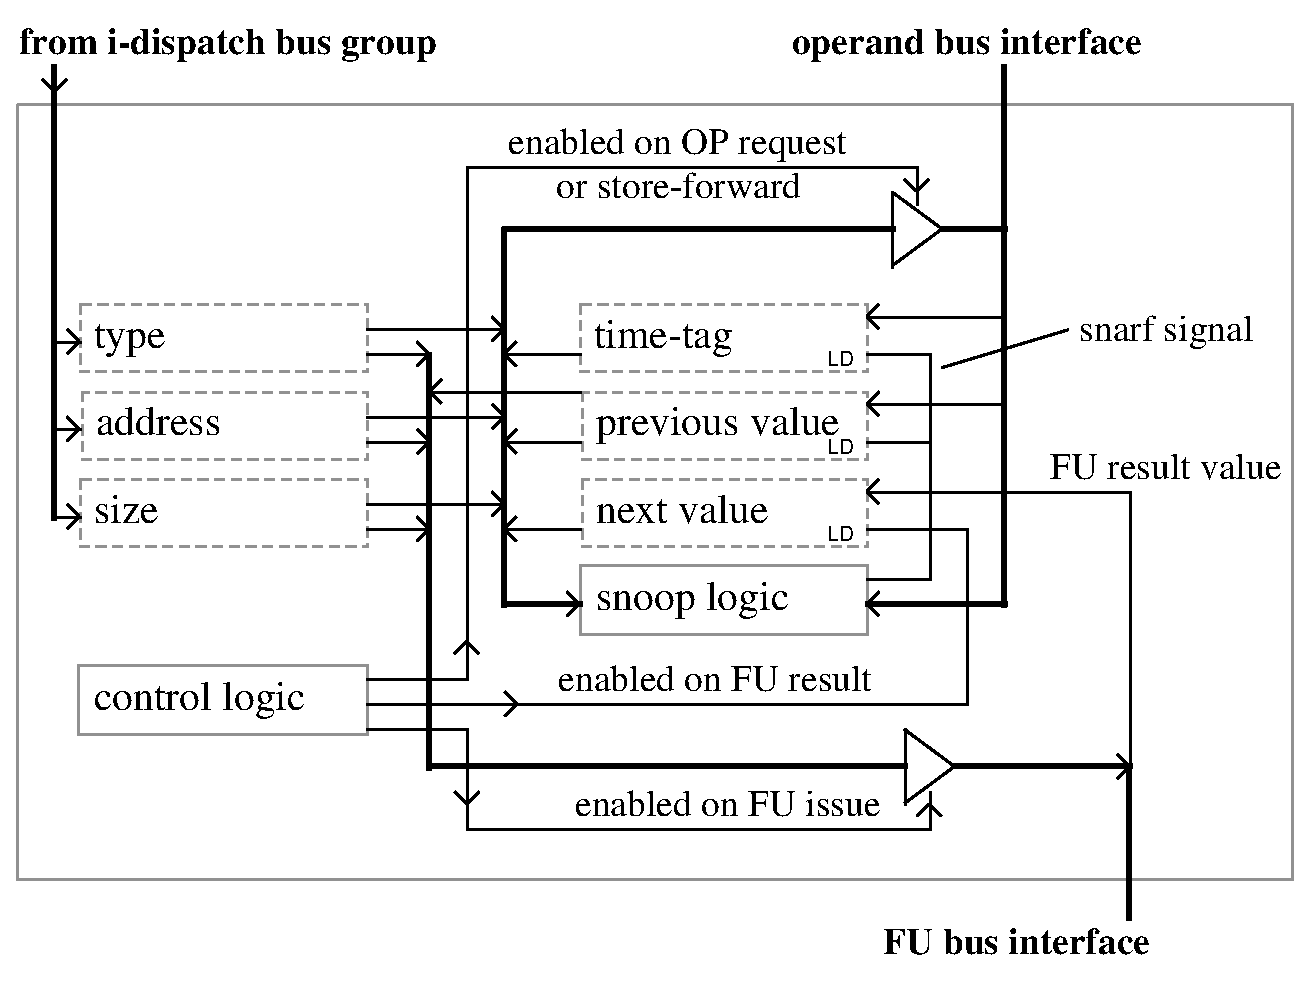
\epsfig{file=figure3.eps,width=3.0in}
\caption{{\em Block diagram of an Operand Block.} 
\small{
Each Operand Block holds an effectively renamed 
operand within the Issue Stations.
Several operand blocks are employed within each Issue Station
depending on the needs of the ISA being implemented.
The primary state register information maintained for each operand (shown in
dash-lined boxes)
along with the major data paths and enabling signals for
its major functions are shown.
}
}
\label{fig:operand}
\end{figure}
%
In effect, a full renaming of
all operands is realized for all instructions
in flight in the machine.  
All false dependencies are thusly avoided.
Full names for operands consist of the components:
%
\begin{itemize}
\vspace{-0.10in}
\item{type of operand}
\vspace{-0.10in}
\item{time-tag}
\vspace{-0.10in}
\item{address}
\vspace{-0.10in}
\end{itemize}   
%
and these components, taken together, fully disambiguate 
all in-flight operands from each other (implementing full renaming).
%
%
%\vspace{-0.25in}
\subsection{Operand forwarding and snooping}
%\vspace{-0.15in}
%
Operands resulting from the execution of instructions
are transmitted forward, using the forward-store bus group,
or use by younger (in program order) waiting instructions.
All forwarded operands are snooped by the operand blocks
within those ISs containing younger dispatched instructions.
The information associated with each operand that is
forwarded is referred
to as a {\em transaction} and consists of:
%
\begin{itemize}
\vspace{-0.10in}
\item{transaction type}
\vspace{-0.10in}
\item{operand type}
\vspace{-0.10in}
\item{address}
\vspace{-0.10in}
\item{time-tag of the originating issue station}
\vspace{-0.10in}
\item{data value for this operand}
\vspace{-0.10in}
\end{itemize}   
%
The time-tag forwarded with the operand is that of the originating
IS (instruction instance).
The operand information above is typical of both
register and memory operand transactions and the use
of the \textit{operand type} distinguishes one from the other.
The \textit{transaction type} field is used to 
designate whether the transaction represents a store from
a previous instruction or an indication that
a previously forwarded operand is no longer valid.

When a set of matching conditions is found by examining the
component parts of the operand while snooping, an acquisition
of the operand is then effected.  
That acquisition is termed a \textit{snarf}.
A snarf for a particular operand
within an IS occurs when: the operand type and address
of the snooped operand match that of the stored operand, and
the snooped time-tag is both less than the current instruction
time-tag (stored in the IS) and is less than or
equal to the last time-tag snarfed for the given stored operand.
In the case of a snarf, the stored operand time-tag (TT) and
previous-value (PV) registers are reloaded with the associated
fields from the snooped operand transaction.
Additionally, if the snooped operand data value is different
than the stored operand previous-value, an execution or a re-execution
is scheduled for the current IS.
However, if the snooped data value is the same as the stored
previous-value, no new execution is triggered.
This eliminates some unnecessary re-executions.

A simplified schematic diagram of the logic used for operand snooping
is shown in Figure \ref{fig:source}.
The {\em time-tag} and
{\em previous-value} registers within an operand block
are reloaded with new values on each snarf,
while the
{\em instruction time-tag} register in the IS
is only loaded when an instruction is dispatched.
The operand block {\em address} register is either loaded at instruction
dispatch or may be loaded during instruction execution for some
instructions
(for example by load-store instructions).
%
\begin{figure}
\centering
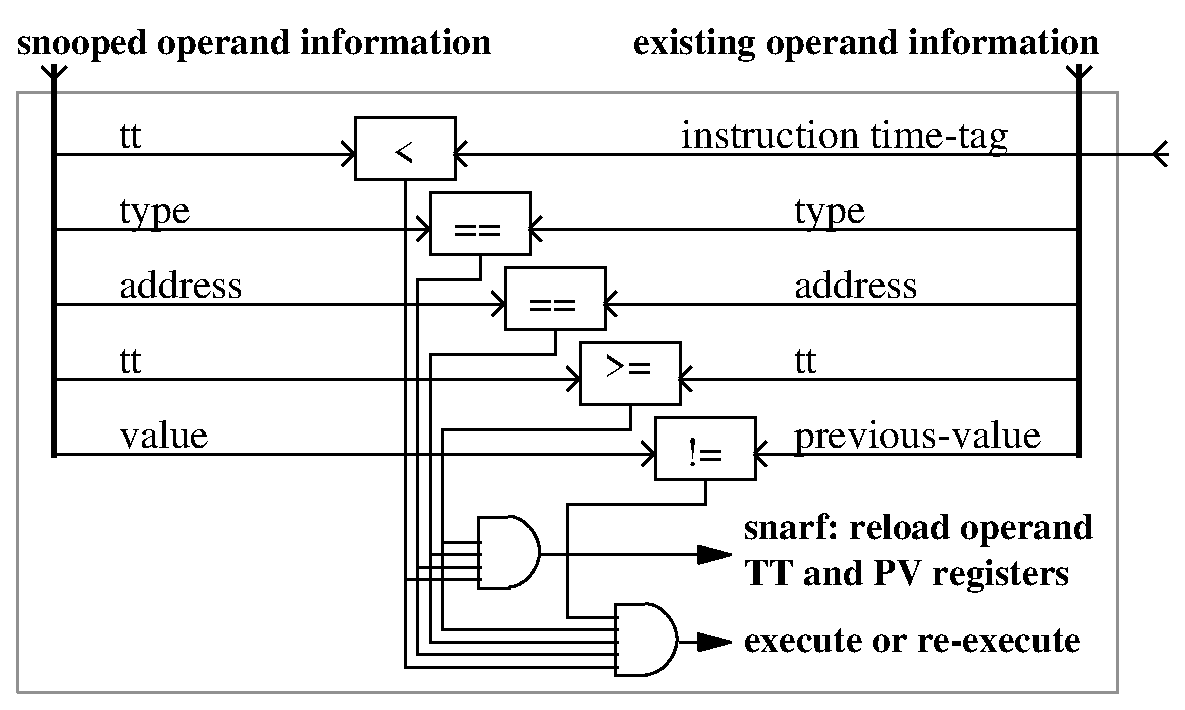
\epsfig{file=figure4.eps,width=3.0in}
\caption{{\em Snooping logic for operand updates.} 
\small{
The snooping
logic for one of several possible source operands is shown.
This logic would reside in each of the operand blocks within an 
IS and they would all perform the snoop operation
simultaneously.
Just one operand forwarding bus is shown being snooped but
typically several forwarding buses are snooped simultaneously.
}
}
\label{fig:source}
\end{figure}
%
Note also that very similar snooping logic is located in
both the LSQ and the architected register file allowing
them to discover operand requests so that they can likewise respond
as ISs do.
%
%
\vspace{-0.15in}
%\vspace{-0.25in}
\section{Experimental results}
%\vspace{-0.15in}
%
In this section we present a first look at some
experimental results from simulation
of the machine presented.
We designed a simulator to evaluate the performance
and characteristics of out proposed design.
The simulator models the major machine components mostly behaviorally
but with the same state and state transitions that would be
in actual hardware.  Components are then interconnected 
structurally.  The simulator implements the Alpha ISA.

We use ten of Spec2000 integer benchmarks 
(listed in Table ~\ref{tab:results} below) to evaluate the potential
of this microarchitecture~\footnote{We have not yet adequately handled
the system calls in the remaining two programs of the SpecInt-2000 suite.}.
For all simulations, the initialization phases of all
programs are skipped using a fast-forward mechanism.
This allows the subsequent functional simulation (which takes
the real bulk of simulation time) to operate on the most
characteristic part of the benchmarks.
After the initial fast-forward operation, a phase of one million 
instructions are executed to warm up machine components that have longer
state residency times.  This currently includes the cache hierarchy
(L1 and L2 caches) and the branch predictor.
Then a short sequence of instructions are 
executed to prime machine components such as the ISs.
This sequence is approximately equal to two times the number
of ISs configured for the target machine.
Finally, we execute on the main functional cycle simulator
for the next 100 million instructions.  

For all simulations, we used separate instruction and
data L1 caches, but a unified L2 cache.
The data caches use a write-back policy with a least recently used
block replacement algorithm.
Other configuration parameters of the machine for the
simulations are shown in Table~\ref{tab:baseline}.

%
\begin{table}
\begin{center}
\caption{{\em General machine characteristics.}
\small{
These machine parameters are used for all simulations
unless otherwise specified.
}
}
\label{tab:baseline}
\scriptsize{
\begin{tabular}{|l|l|}
\hline 
L1 I cache access latency&1 clock\\
\hline
L1 I cache size&32 KBytes\\
\hline
L1 I block size&32 bytes\\
\hline
L1 I organization&direct mapped\\
%
\hline 
L1 D cache access latency&2 clocks\\
\hline
L1 D cache size&128 KBytes\\
\hline
L1 D block size&32 bytes\\
\hline
L1 D organization&2-way set assoc.\\
%
\hline
L2 cache access latency&20 clocks\\
\hline
L2 cache size&1 MBytes\\
\hline
L2 block size&32 bytes\\
\hline
L2 organization&4-way set assoc.\\
%
\hline
main memory access latency&150 clocks\\
\hline
branch predictor&2-level w/ XOR\\
\cline{2-2}
 & 16k PHT entries\\
\cline{2-2}
 & 8 history bits\\
\cline{2-2}
 & 32k BHT entries\\
\cline{2-2}
 & sat. 2-bit counter\\
\hline
fetch width & 8 instructions \\
\hline
FU issue width & 4 operations \\
\hline
issue width & 4 \\
\hline
number integer FUs & 4 \\
\hline
number other FUs & 1 each \\
\hline
forwarding buses & 8 \\
\hline
bus traversal latency & 1 clock \\
\hline
integer FU latency & 1 clock \\
\hline
other FU latencies & 3 to 17 clocks \\
\hline 
\end{tabular}
}
\end{center}
\end{table}
%

We present the IPC results of our proposed
microarchitecture with that of a baseline 
superscalar microarchitecture that is similarly configured.
We used the 
Simplescalar MASE framework~\cite{Austin97}
to simulate a conventional superscalar (approximately a MIPS R10000
in the case of SimpleScalar MASE).

The baseline superscalar machine includes an instruction
window consisting of reservation stations and a re-order buffer (ROB)
to store speculative execution result registers pending commitment.
Instructions for the baseline superscalar are fetched and dispatched
to the instruction window where they wait for input data dependencies to
become ready.  When all instruction input dependencies are ready,
and as issue bandwidth allows, instructions are issued to the
function-unit pipelines.  Register results are stored in the ROB
until commitment.  
Both the baseline superscalar and our proposed
microarchitecture flush the execution window on a resolved mispredicted 
conditional branch.
This is a fairly typical superscalar execution
arrangement and is fixed in the Simplescalar MASE simulator.

Although an exact comparison of the two machines is not possible
due to their very different construction, we have arranged
for both the baseline machine and our proposal to have either an
exact or a very
close correspondence in the amount and number of hardware resources.
Both machines are configured with identical
cache arrangements and cache configurations.
Both also employ the same branch predictor and predictor configuration.
Both also implement a four-wide issue machine.
For both machines, the issue width is the maximum number of
instructions that can be issued in a single clock cycle.
However the baseline superscalar employs reservation stations and
an ROB while our microarchitecture uses our novel ISs.
We therefore roughly equate the number of ISs of
the proposed machine with the combination of both the
number of instruction window slots (reservation stations)
and ROB entries of the baseline superscalar.
Our results are for 128 ISs in the proposed 
microarchitecture and both 128 issue window slots (reservation stations)
and 128 ROB entries for the baseline superscalar.
This represents a modest sized machine of today.

The IPC results for the baseline superscalar and our proposed
machine are shown in columns two and three of Table~\ref{tab:results}
respectively.
In order to get a feel for how much re-execution of instructions
occurs, we also list in the results (in column 4 labeled REX)
the percent additional instructions
executed as compared with the number of committed 
instructions.
We also calculated the harmonic mean of the IPC
across all benchmarks (last entry in table).
Columns 5 is discussed later.
%
\begin{table}[t]
\begin{center}
\caption{{\em IPC and re-execution results.}
\small{
IPC performance of a MASE baseline superscalar machine and our
proposed microarchitecture is presented.
The column titled REX gives the percent of 
extra instructions executed for the newly proposed machine as compared with 
the committed instructions.
}
}
\label{tab:results}
\vspace{+0.1in}
\scriptsize {
\begin{tabular}{|l||r|r|r|r|}
\hline
 & baseline &
 \multicolumn{2}{c|}{new} &
 {new-extra} \\
\cline{2-5}
 & IPC & IPC & REX & IPC \\

\hline
\hline
bzip2&
2.11 & 1.98 & 97.8\% & 2.41 \\

\hline
crafty&
1.34 & 1.96 & 79.2\% & 2.33 \\

\hline
eon&
1.25 & 2.62 & 110.4\% & 3.12 \\

\hline
gcc&
1.32 & 1.70 & 96.2\% & 2.41 \\

\hline
gzip&
1.35 & 1.42 & 98.0\% & 1.93 \\

\hline
parser&
0.80 & 1.23 & 115.8\% & 1.41 \\

\hline
perlbmk&
0.64 & 1.44 & 92.3\% & 1.52 \\

\hline
twolf&
1.16 & 1.32 & 88.2\% & 1.60 \\

\hline
vortex&
1.05 & 2.61 & 103.7\% & 3.75 \\

\hline
vpr&
1.08 & 1.13 & 96.1\% & 1.39 \\

\hline
\hline
H-MEAN&
1.10 & 1.61 & & 1.97 \\

\hline
\end{tabular}
}
\end{center}
\end{table}
%
Comparing the harmonic mean IPC results in columns two and three of the
Table~\ref{tab:results} (last entry), 
our proposed machine attained a speedup (1.61 divided by 1.10) 
of approximately
1.46 as compared with the baseline superscalar.
This was achieved using approximately the same amount of hardware resources.
All individual programs performed better with the exception of
the BIPZ2 program.
We are still exploring why BZIP2 performed poorly on our
machine as compared with the baseline superscalar.
We have not found any single internal metric that seems to
present a particular bottleneck for BZIP2, but it also may be that
some feature of the conventional machine allowed it to perform
unusually well for some reason.
Column 4 of Table~\ref{tab:results} (titled REX) shows the percentage
of committed instructions that incurred re-executions.
Most benchmarks exhibit a behavior of executing somewhere around
200\% (within about plus or minus 20\%) of the committed
number of instructions.
This compares similarly to the amount of execution needed
in proposals like the SlipStream processor~\cite{ibrahim03},
except that neither two threads nor two processors need be
dedicated to the execution of a single program, as it done in
that processor. 
Rather, approximately two times the execution was performed
within the resources of a single core and threaded machine.

Column 5 provides the IPC results for a version of the
machine where additional instructions are executed within
the ISs as compared with the machine of column 3.
Minimally, control-flow and memory load-store instructions
are executed in the ISs.  
However with a very small additional amount of silicon,
simple bit-logic instructions and integer add and subtract
instructions (including integer compare) can also 
be executed within the ISs.
This arrangement (transistors permitting) increases the
amount of resources available for executions, thus increasing
parallelism and IPC performance.
This yields approximately 22\% better IPC performance
than with the minimal configuration proposed machine, and approximately
79\% IPC improvement of the baseline machine.

We note that with a higher IPC, 
power consumption can be reduced while achieving the same
performance as the baseline machine by lowering clock frequency.
Future research might also realize power savings through the possible
elimination of redundant re-executions.
%
%
\vspace{-0.15in}
%\vspace{-0.25in}
\section{Summary}
%\vspace{-0.15in}
%
We have described a new microarchitecture that
allows for both control and data speculative execution,
but also does so 
in a way where necessary re-executions are handled
quickly and cheaply in the hardware, without requiring either
re-fetch or re-dispatch.  
The necessary and complicated instruction dependency
enforcement is achieved dynamically during execution (and re-execution)
using time-ordering tags that maintain relative program order
of instructions and all operands in flight.
Binary program compatibility with existing ISAs (an important feature
in the market place) is also maintained with our proposal.
Our results show that our proposed machine achieves approximately
46\% better IPC performance over a conventional machine of roughly
equivalent silicon resources, and approximately a 79\%
IPC improvement given some modest additional silicon to facilitate
executing additional instructions in the issue stations.
Physical scalability is possibly facilitated due to the distributed
handling of operand dependency determination and forwarding.
%
\bibliographystyle{latex8}
\bibliography{flowing}
%
\end{document}
%
%
%
